\documentclass[12pt,a5]{bxjsarticle}

\usepackage{xltxtra}
\setmainfont{IPAPMincho}
\setsansfont{IPAPGothic}
\setmonofont{IPAGothic}
\XeTeXlinebreaklocale "ja"

\usepackage{hyperref}
\usepackage{listings}
\usepackage{verbatim}
\usepackage{bm}

\newcommand{\e}{\mathrm{e}}

\title{物理学情報処理論2 problem6}
\date{}

\begin{document}
\maketitle

\section{}
3次元空間内で、荷電粒子の運動について、
\[
\frac{d^2\bm{r}}{dt^2} = \frac{1}{r^3}(\frac{d\bm{r}}{dt} \times \bm{r})
\]
において、
\[
\bm{r}(t) = \left[
  \begin{array}{c}
    x(t) \\
    y(t) \\
    z(t)
  \end{array}
\right],
\frac{d\bm{r}}{dt}(t) = \left[
  \begin{array}{c}
    u(t) \\
    v(t) \\
    w(t)
  \end{array}
\right]
\]
とおいて、初期条件を$ (x(0), y(0), z(0)) = (1, 0, 0), (u(0), v(0), w(0)) = (-1, v_0, 0) $とする。

このとき、$ v_0 $として$v_0 = 0.01, 0.1, 0.3, 0.5 $として数値的に軌道を求めたのが、以下のグラフである。
この際Symplectic法にて数値的に計算した。

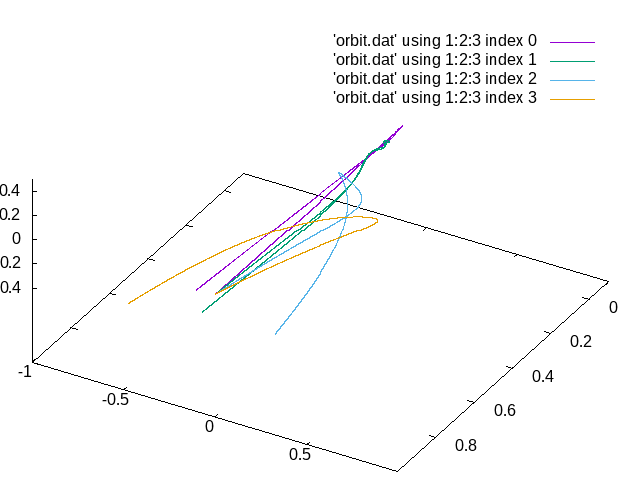
\includegraphics[width=\linewidth]{orbit.png}

粒子の軌道で原点と最も近い距離のプロットと、$v_0/sqrt{1+v_0^2}$のグラフが以下である。

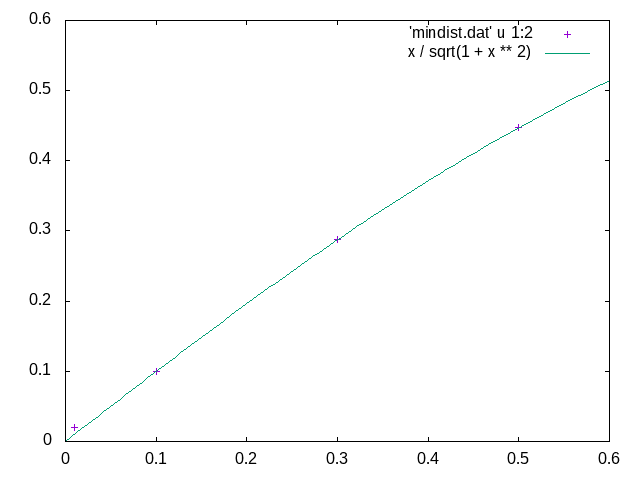
\includegraphics[width=\linewidth]{min.png}


以下のスクリプトを用いて、orbit.datから図を生成した。
\lstinputlisting[caption=plot.sh,language=bash]{plot.sh}

\end{document}
